%!TEX root = ../Dokumentation.tex

\section{RESTful Webservice}

\subsection{Vertiefung}

Nach der konzeptionellen Planung der Ressourcen und HTTP - Operationen, geht es um die codebasierte Umsetzung. Definierte XML Schemas werden nach erfolgreicher Validierung in JAXB Objekte überführt, um eine Verwendung des Datenbestandes im Javaprojekt zu ermöglichen und aus den Schemadateien Java-Klassen zu erzeugen.\\
Zur Realisierung der synchronen Kommunikation wird Grizzly als Webserver der HTTP - Operationen verwendet. Zusätzlich wird zur Entwicklung des RESTful Webservices das Jersey framework implementiert, dass für JAX-RS APIs und Server als Referenzimplementierung dient.\\
\vspace{0.2cm}
Bereits im Rahmen der Ressourcenfindung, wurde sich Gedanken darüber gemacht, wie URI zur jeweiligen Ressource gestaltet werden können, damit ein logischer Request auf gewünschte Daten stattfinden kann.\\
Die Repräsentation einer spezifischen Ressource wurde im vorherigen Abschnitt mittels \textbf{Path-Parameter} realisiert, das heißt, der Parameter ID war Teil der eigentlichen URI.\\
Als Alternative können allerdings auch sogenannte \textbf{Query-Parameter} zum Einsatz kommen. Diese eignen sich meistens um Ressourcen noch weiter zu verfeinern und sind in der Regel optional.\\

Innerhalb des Serientrackers hat man es grundlegend mit 2 Typen von Daten zu tun, die bereits in vorherigen Überlegungen angesprochen wurden.Zum einen haben wir feste Objekte wie Serien, Season oder Episoden, die eine eindeutige ID erhalten und sich über diese auffinden lassen. Für diese Typen eignet sich besonders die Path-Parameter Anfrage.
Diese Zeichnen sich durch die einfach Angabe des Pfades aus wie beispielsweise \textbf{@Path( "{serieID}" )} für die GET Operation auf die URI \textit{/series/\{serieID\}}.\\
Der zweite Typ sind die jeweiligen Listen, die sich durch die Elemente und Attribute der Serien entsprechend kategorisieren lassen. Eine Konzeptidee war das Abonnieren bestimmter Genres. Da Listen aber generell Serien unterschiedlichen Genres aufnehmen können, prinzipiell aber auf dem selben XML Schema \textit{list} beruhen, wurde nach einer Möglichkeit entsprechende Objekte bei einem Request herauszufiltern.\\ Die Lösung dieses Problem wurde dann über eine Erweiterung der XSD, sowie der Abfrage per Query-Parameter innerhalb des ListsService erzielt.
\newpage
\begin{lstlisting}[basicstyle=\ttfamily,numbers=left,numberstyle=\footnotesize\ttfamily,backgroundcolor=\color{source},label=listsservice,caption=Auszug aus ListsService mit QueryParam]
@Path( "/lists" )
public class ListsService {

@GET
  @Produces( MediaType.APPLICATION_XML )
  public Response getGenreList(
                @QueryParam( "type" ) String type,
                @QueryParam( "name" ) String name)
  [...]
\end{lstlisting}

Als zusätzliche Parameter dienen hierbei \textit{type} zur Abfrage, ob es sich um einer Userliste oder Genreliste handelt und der entsprechende \textit{name} der Liste, falls es eine Genreliste ist.
Genrelisten weisen hierbei nur Serien eines bestimmten Typs auf und werden speziell für diesen Zweck angelegt. Eine Abfrage auf diesen Typ erhält die Form \textsf{/lists/?type=genre\&name=action} und würde bei erfolgreichem Request die entsprechende Liste mit den Serien vom Genre Action zurückgeben.
\\
Weiterhin könnte exemplarisch  ein Query-Parameter in diesem Projekt bei der Ressource Users zum Einsatz kommen, um nur die Benutzer der Gruppe Admin zu repräsentieren:\\ \textsf{/users/?group=admins}. Aber auch bei einem Zugriff auf eine einzelnen Episode einer Staffel einer Serie können Query-Parameter genutzt werden, Beispiel: \textsf{/episodes/?serie\_id=1\&season\_id=2}. Jedoch wären die Parameter an dieser Stelle obligatorisch.
\\
Als Alternative zu den beiden Varianten bietet sich noch der \textbf{HTTP-Header} des Clienten an. Da diese Art von Parameterübertragung eher untypisch ist, wird an dieser Stelle nicht weiter drauf eingegangen.

\vspace{0.2cm}

Da jeder Request auch immer einen Response erfordert, ist es bei der Umsetzung notwendig, Statuscodes der HTTP - Operationen zu benutzen. Dabei viel die Wahl auf folgende Statuscodes bei zugehörigen Ereignissen.

\begin{table}[H]
\caption{Statuscodes der Webservice Ressourcen}

\centering
\begin{tabular}{l l l}
\\ [-0.5ex]

\hline\hline
\\ [-0.5ex]
Statuscode & Bedeutung
\\ [1.5ex]
\hline
\\ [-0.5ex]
400 & Bad Request - Request konnte aufgrund der Syntax nicht verstanden werden\\[1ex]
404 & Not Found - kein passender Treffer in der gefragten Ressource-URI \\[1ex]
409 & Conflict - Request aufgrund aktuellen Status nicht ausführbar\\[1ex]
500 & Internal Server Error - unerwartete Umstand, Request nicht durchgeführt\\[1ex]

\hline
\end{tabular}
\label{tab:statuscodes}
\end{table}

Wie diese Codes innerhalb der einzelnen Response-Methoden Verwendung finden, wird im folgenden an Beispielen dargestellt. Nach einigen Vorüberlegungen folgt nun die Umsetzung in Java und das finale Ergebnis.

\subsection{Umsetzung}

Aufbauend auf die zuvor identifizierten URI, ging es nun darum die HTTP Methoden auf die einzelnen Ressourcen umzusetzen. Aus struktureller Sicht wurde dabei für jede Ressource eine eigene Service-Klasse angelegt, welche die jeweiligen Operationen bereitstellt. Innerhalb einer solchen, werden angedachte URI Pfade der Tiefe nach implementiert. Das Prinzip verdeutlicht folgende Übersicht zum Klassenaufbau des SeriesService und SeasonService:

\begin{lstlisting}[label=seriesseasonsservices,caption= Klassenaufbau von BeispielServices]
/**
 * Service for:
 * GET     /series
 * POST    /series
 * GET     /series/{serieID}
 * DELETE  /series/{serieID}
 * PUT     /series/{serieID}
 * GET     /series/{serieID}/seaons
 * GET     /series/{serieID}/seaons/{seaonID}
 * GET     /series/{serieID}/seaons/{seaonID}/episodes
 * GET     /series/{serieID}/seaons/{seaonID}/episodes/{episodeID}
 */
@Path( "/series" )
public class SeriesService {}

/**
 * Service for:
 * GET     /seasons
 * POST    /seasons
 * GET     /seasons/{seasonID}
 * DELETE  /seasons/{seasonID}
 * PUT     /seasons/{seasonID}
 */

 @Path( "/seasons" )
public class SeasonsService {}

\end{lstlisting}
Wie bereits angesprochen, bestand die Möglichkeit zum Season und Episoden Zugriff auf unterschiedliche Wege. Da für jeden dieser Services eine mehrfache Definition aller Methoden nicht notwendig oder sinnvoll ist, wurde sich für eine Art Mittelweg entschieden. Die aufeinander aufbauende Variante im oberen Beispiel des SeriesService, erschien in sofern reizvoll, die die eindeutige Abfrage einer Episode über den jeweiligen Pfad realisiert werden könnte. Die zweite Variante stellt dabei eine höhere Komfortabilität dar, da zum Abrufen einer Season keine Serie ID bekannt sein müsste (die durch die XSD Definition jedoch vorhanden ist).\\
Daher wurden geplante POST, PUT und DELETE Methoden, jeweils nur auf den Haupttyp definierte und der Pfadzugriff in die Tiefe ermöglicht lediglich ein Holen der Daten, keine Manipulation. Diese sind in der jeweiligen Serviceklasse realisiert.

\vspace{0.2cm}

Zu Beginn wurden einzelne Methoden ausgearbeitet und auf Funktionalität in Verbindung mit dem Grizzly RESTServer getestet. Erste Versuche wurden mit Hilfe eines erstellten TestClients durchgeführt und lieferten schnell das gewünschte Ergebnis.\\
Innerhalb dieser Phase fand  die gesamte Realisierung in der jeweiligen Methode definiert. So wurde beispielsweise das Marshalling und Unmarshalling jedes Mal erneut eingebunden.

\begin{lstlisting}[label=getsingleseriesservice,caption= GET Testmethode der SeriesID]
   @Path( "/{id}" )
   @GET @Produces( "application/xml" )
   public Serie getSingle(@PathParam("id") int id) throws JAXBException {
       ObjectFactory of = new ObjectFactory();
       Series series = of.createSeries();
       JAXBContext jaxbContext = JAXBContext.newInstance( Series.class );

       this.unMarshaller = jaxbContext.createUnmarshaller(); // Reading
       Series rawSeries = (Series) unMarshaller.unmarshal( this.file );

       List<Serie> series = rawSeries.getSerie();
         for ( Serie serie : series ) {
            if ( serie.getSerieID().intValue() == id ) {
                return serie;
            }
        }
   return null;}
\end{lstlisting}
\begin{lstlisting}[label=testclient,caption= Anfrage des Testclients nach Serie mit angegebener ID]
public static void testGetSerie() {
    String url = host + "/series/ss_0001wade";
    System.out.println( "GET: " + url );
    WebResource wrs = Client.create().resource( url );

    ClientResponse response = wrs
        .accept( MediaType.APPLICATION_XML )
        .get( ClientResponse.class );

    if ( response.getStatus() != 200 ) {
      System.err.println( "Failed: HTTP error code: " + response.getStatus() );
      return;
    }
    Serie output = response.getEntity( Serie.class );
    System.out.println( "Output from Server..." );
    System.out.println( output.getTitle() );
  }
\end{lstlisting}

Eine Abfrage der Liste lieferte im Idealfall das gesuchte Objekte.So ermöglichte obige Anfrage die Rückgabe der Serie mit angegebener ID.\\
Da diese Herangehensweise aus programmiertechnischer Sicht jedoch nicht besonderns effektiv und angebracht ist, fand im weiteren ein Refactoring des Webservices statt und der Klassenaufbau wurde angepasst. Ganz nach dem DRY Prinzip (don't repeat yourself) wurden wiederkehrende Informationen, wie das zuvor angesprochene Marshalling und Unmarshalling, auf eine eigene Klasse ausgelagert um Coderedundanz zu vermeiden und definierte Funktionen an mehreren Stellen zugänglich zu machen. Während der Entwicklung ergab sich daraus folgender Aufbau, bei dem einzelne Komponenten funktional miteinander Interagieren und im Zusammenspiel die synchrone Kommunikation des SerienTrackers ermöglichen.

\begin{figure}[h!]
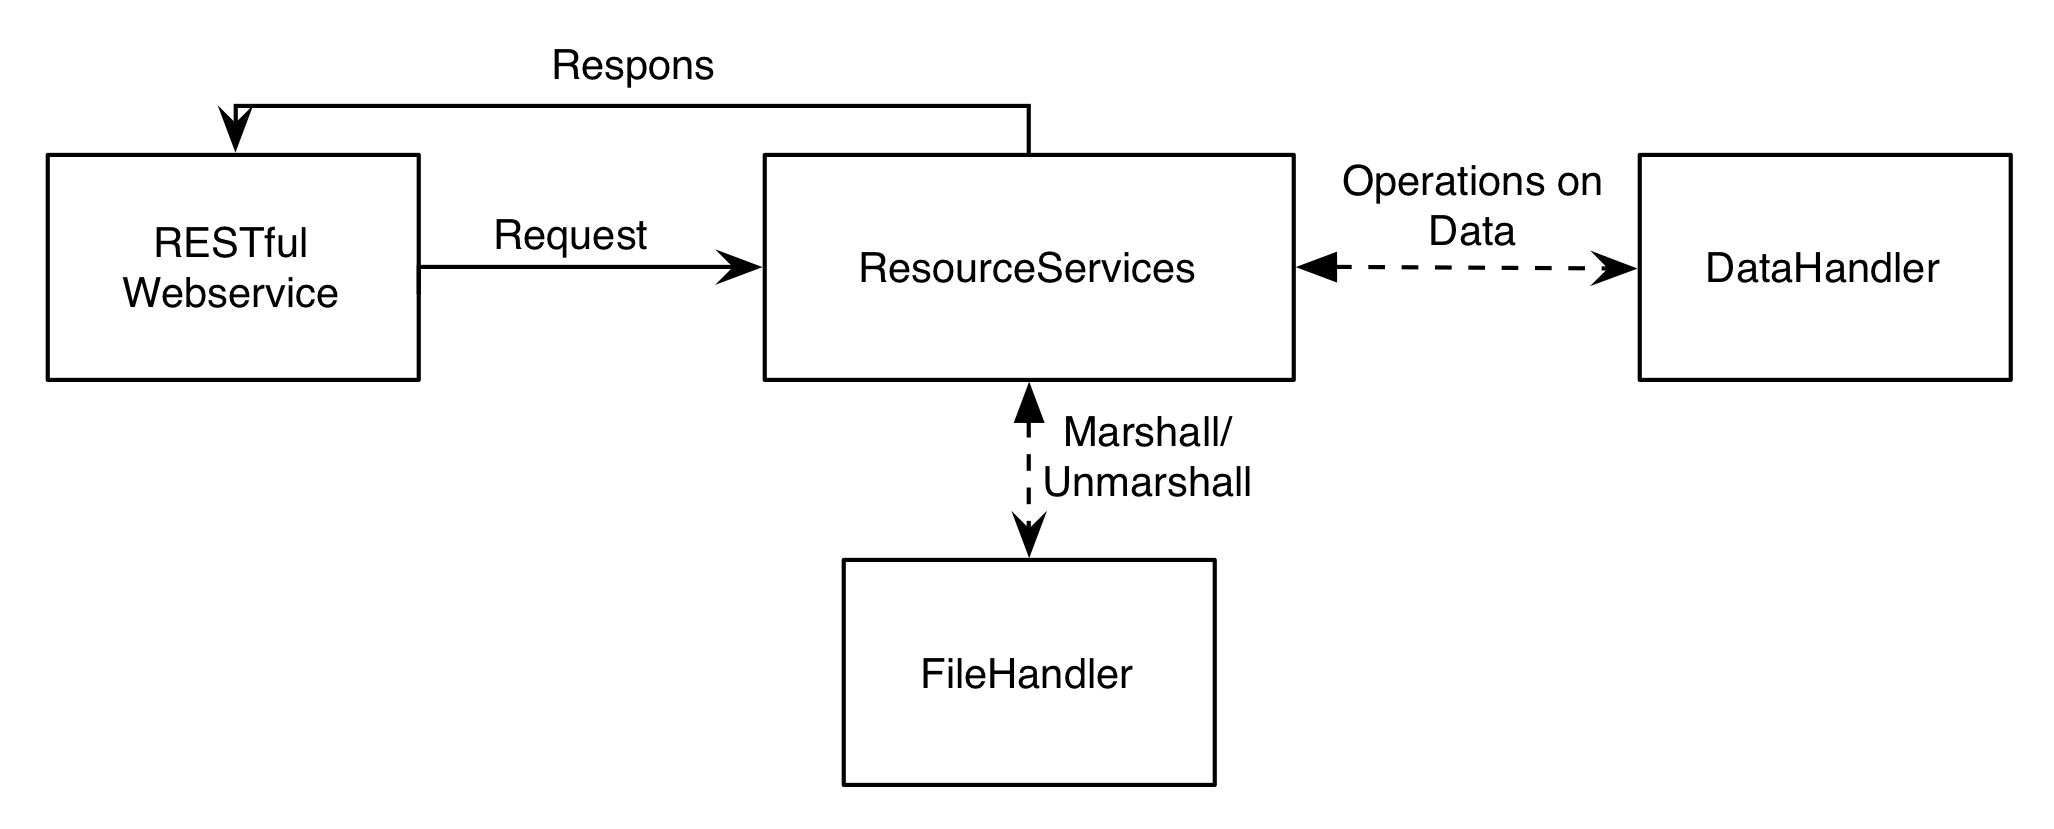
\includegraphics[width=1\textwidth]{../images/aufbaurest.png}
\caption{Funktionaler Aufbau der Komponenten zur synchrone Kommunikation }
\label{RESTaufbau}
\end{figure}

Über den RESTServer wird ein Request an die Serviceklasse einer Ressource geschickt. Die angesprochene Methode beginnt die Anfrageverabeitung und wird zuerst durch einen Logger erfasst \textit{  Logger.log( ... );}. Diese Hilfsklasse wurde erstellt, um während der Entwicklung einzelne Schritte zu dokumentieren und erfolgreiche und nicht erfolgreiche Arbeitsschritte genauer bestimmen zu können. Die Serviceklasse greift dann gegebenfalls auf Methoden des FileHandlers und DataHandlers zu. Klassen in denen jeweilige Funktionen ausgelagert wurden. Der FileHandler kümmert sich um das Lesen und Schreiben der Daten in die XML Files durch Marshalling und Unmarshalling Operationen. Zudem überprüft sie, ob für entsprechende Objekte bereits XML Files zu Grunde liegen, ansonsten werden diese neu erstellt.\\
Der DataHandler stellt die Methoden bereit, um auf vorhandene Daten zu operieren und den jeweiligen Request funktional umzusetzen. So wird biespielsweise ein Serienobjekt in der SeriesServiceklasse erstellt und durch eine Methode des Handlers \textit{Serie serie = dh.getSerieByID( id );} durchsucht der zugehörige SeriesDataHandler  vorhandene Elemente nach dem passenden Attribut und liefert die gesuchte Instanz zurück. Der Rückgabewert wird dann wieder vom Service geprüft und per Response zurückgeliefert. Gegebensfalls folgt die Rückgabe eines Statuscodes beim Eintreten eines des darin beschriebenen Ereignisses.\\
Die DataHandler wurden entsprechende der persistende Datenstruktur in die jeweiligen Typen aufgeteilt und übernehmen für zugehörige Ressourcen die Verarbeitung. Dadurch entwickelte sich der SeriesDataHandler, UsersDataHandler und ListsDataHandler. Im momentanen Entwicklungsstand des Projektes, verarbeitet der SeriesDataHandler vorerst auch nur die Informationen einer Serie.

\vspace{0.2cm}
Entsprechende Unterstützung einer Season oder Episode nach diesem Prinzip ist aus zeitlichen Gründen noch nicht implementiert, die Funktionalität der entsprechenden HTTP Operation findet noch auf eine andere Weise statt. Entsprechende GET Anweisungen könnten über die \textit{series/{serieID}/seasons/{seasonID}/episodes} - URI ermöglicht werden. POST, PUT und DELETE Methoden sind innerhalb der Services umgesetzt.\\
Die Kommunikation zwischen Client und Server ermöglicht bisher einen Austausch zwischen den Serien und Userdaten. In Bezug auf Serien, wurde ein ListService erarbeitet, der jedoch noch nicht auf Funktionalität getestet werden konnte, da der zugehörige ListDataHandler noch Probleme aufweist. Für eine Lösung dieses Problems wäre dabei die Anpassung im Stile des UsersDataHandlers möglich. Dieser greift auf entsprechenden Fileordner auf der Database zu um die passende Userdatei zu erhalten oder legt alternativ neue Files für die einzelnen User an. Der ListsDataHandler geht diesen Schritt etwas anders an, indem er auf die lists.xml zugreift. Auch hier müsste ein Zugriff auf den gesamten Ordner realisiert werden und dann die einzelnen Dateien durchsucht werden. Momentan führt dieser Ansatz nicht zum erwünschten Zweck, da innerhalb der selbstdefinierten Database keine lists.xml existiert, die in der Zeit der Ausarbeitung als Testdatei bestand. Bei der Entwicklung der Testdaten wurde für jede Liste eine seperate Datei angelegt. Eine Zugriff auf eine XML File die mehrere Listen enthält wäre über die genre.xml oder user.xml vorstellbar. Dies wäre ein Grundansatz um dieses Problem entgegen zu gehen. Die entsprechende Pfadauslegung und anschließende Abfrage in Bezug auf die aktuelle Datenstrukturierung.

Zusätzlich zu den Services sei noch erwähnt, dass neben den jeweiligen RessourceServices ein zusätzlicher ImageService entwickelt wurde. Dieser arbeitet ebenfalls unter Verwendung der GET Methode und gibt dabei gespeicherte Bilder nach Filenamen zurück. Die Anwendung dieser Klasse, spielt jedoch erst in der Cliententwicklung eine Rolle.\\
\newpage
Im weiteren Rahmen der Dokumentation soll hierbei nicht auf jede einzelne Klasse eingegangen werden. Für einen kurzen Einblick in die Ausarbeitung, werden deshalb im folgenden nur kurz einzelne Aspekte der verschiedenen Methoden am Beispiel des SeriesService dargestellt.
\begin{lstlisting}[label=getseriesservice,caption= GET Methode /series ]
  @GET
  @Produces( MediaType.APPLICATION_XML )
  public Response getSeries() {
    Logger.log( "GET series called" );
    Series series = dh.getSeries();

    if ( series == null )
      return Response.status( 404 ).build();

    return Response.ok().entity( series ).build();
  }
\end{lstlisting}
Im Vergleich zur vorherigen GET Methode, fällt die gewonnene Überischtlichkeit und Einfachheit auf. Der DataHandler dh führt die eigentliche Operation aus und liefert in dem Fall alle Serien zurück die vorhanden sind. Sind keine Serien auffindbar, wird der NOT FOUND Statuscode 404 als Response zurückgegeben. Bei Erfolg die gefundenen Entitäten.
\begin{lstlisting}[label=addseriesservice,caption= POST Methode /series ]
@POST
  @Consumes( MediaType.APPLICATION_XML )
  public Response addSerie( Serie newSerie ) {
    Logger.log( newSerie.getTitle() );

    String id = "ss_" + Hasher.createHash( newSerie.getTitle() );

    if ( dh.SerieExistsByID( id ) )
      return Response.status( 409 ).build();

    newSerie.setSerieID( id );

    if ( ! dh.addSerie( newSerie ) )
      return Response.status( 500 ).build();

    URI location = null;
    try {
      location = new URI( RESTServerConfig.getServerURL() + "/series/" + id );
    } catch ( URISyntaxException e ) {
      e.printStackTrace();
    }
    return Response.created( location ).build();
  }
\end{lstlisting}

Die POST Methode zum Pfad /series erstellt eine neue Serie und fügt sie in die Liste ein. Zuerst wird eine neue ID der Serie erstellt. Dazu wird mit der eigenen Hilfsklasse Hasher eine eindeutige Kennung erstellt, wie sie im Abschnitt zur XML Entwicklung bereits angesprochen wurde. Es folgt die Kontrolle, ob die Serie anhand der ID bereits exisitert, wenn ja wird der 409 Conflict Statuscode ausgegeben, um dies zu vermeiden. Sofern es Probleme beim hinzufügen gab, wird dies vom Statuscode 500 informiert über serverseitige Probleme. An geplanter location im URI Pfad wird das Objekt anschließend erstellt.\\
Auch die beiden weiteren Methoden PUT und DELETE sind nach diesem Prinzip strukturiert. PUT ändert die Daten des bestehenden Objektes zu angegebener ID. Sofern die Serie existiert und Kontrollabfragen keinen Fehlercode zurückgeben, war die Änderung erfolgreich. DELETE entfernt nach gleicher Abfrage das gewünschte Objekte aus vorhandenem Datenbestand.\\

Dieser kurze Einblick in den RESTful Webservice, sollte einen Überblick über die Ausarbeitung der synchronen Kommikationsvorgänge schaffen. \\
Zu Beginn des Projektes wurden in der Konzeptidee diverse Möglichkeiten überlegt, die vom System unterstützt werden können. Für Serieninteressierte wurde beispielsweise das Favorisieren von Serien, Anlegen von Listen oder Markieren und Bewerten von Episoden angedacht. Die Auseinandersetzung mit dem Projekt, zeigte bei diesem Meilenstein, dass dieses Ziel vom entsprechenden Umfang her zu hoch ausgelegt war. Daher wurde der Fokus auf einen Teil dieser Möglichkeiten gelegt und nur ein Teil davon vertieft umgesetzt. Der Aspekt des Favorisieren und die Listen stellten für den weiteren Verlauf den größten Nutzen dar, weil anhand dieser Elemente die entsprechende Benachrichtigung innerhalb der asynchronen Kommunikation realisiert werden kann. Die weiteren Ansätze wurden zugunsten des Projektzieles außen vor gelassen, könnten aber in einem größer angelegten Projekt dieser Art eine Ausbaumöglichkeit darstellen.
